\documentclass[11pt]{beamer}
\usepackage{graphicx}
\graphicspath{ {./Images/} }
\setbeamertemplate{caption}[numbered]
\usepackage{caption}
\usepackage{float}
\usepackage{hyperref}
\usepackage{multirow}
\setbeamersize{text margin left=0.5cm,text margin right=0.5cm}
\usepackage{multicol}
\usepackage{listings}
\usepackage{color}
\usepackage{fancyvrb}
\usepackage{booktabs}
\definecolor{dkgreen}{rgb}{0,0.6,0}
\definecolor{gray}{rgb}{0.5,0.5,0.5}
\definecolor{mauve}{rgb}{0.58,0,0.82}
\lstset{
  language=Java,
  aboveskip=3mm,
  belowskip=3mm,
  showstringspaces=false,
  columns=flexible,
  basicstyle={\small\ttfamily},
  numbers=none,
  frame=single,
  numberstyle=\tiny\color{gray},
  keywordstyle=\color{blue},
  commentstyle=\color{dkgreen},
  stringstyle=\color{mauve},
  breaklines=true,
  breakatwhitespace=true,
  tabsize=3,
  fancyvrb=true,
}
\makeatletter
\let\save@measuring@true\measuring@true
\def\measuring@true{%
  \save@measuring@true
  \def\beamer@sortzero##1{\beamer@ifnextcharospec{\beamer@sortzeroread{##1}}{}}%
  \def\beamer@sortzeroread##1<##2>{}%
  \def\beamer@finalnospec{}%
}
\makeatother
\mode<presentation> {
    \usetheme{Warsaw}
    \setbeamertemplate{footline}[page number]
    }    
\definecolor{violet}{rgb}{0.54, 0.17, 0.89}
\newcommand{\red}[1]{\textcolor{red}{#1}}
\newcommand{\violet}[1]{\textcolor{violet}{#1}}
\newcommand{\green}[1]{\textcolor{green}{#1}}
\newcommand{\sol}{\textbf{Solution}: \pause \newline}

\title[Chapter 04 Notes]{Math 130: Introduction to Programming \\ Chapter 04: Loops and Files \\ Lecture Notes}
\author{Jesús R. Pérez Cuarenta \\
	\href{mailto:jperezcuarenta@swccd.edu}{jperezcuarenta@swccd.edu}
	}
\date{}

\begin{document}
\section{}
\begin{frame}
  \maketitle
\end{frame}

\begin{frame}
\frametitle{Overview}
    \begin{multicols}{2}
    \tableofcontents
    \end{multicols}
\end{frame}

\section{Increment}
\subsection{Increment and Decrement Operators}
\begin{frame}{Increment and Decrement Operators}
    Before getting into loops, we'll briefly cover the \violet{increment (++)} and \violet{decrement (--)} operators. These operators can increase and decrease the value of a variable by one. Both update the value of the operand to its new value. They have two forms: prefix and postfix.
\end{frame}

\subsection{Prefix and postfix}
\begin{frame}[fragile]{Pre-increment and pre-decrement}
    To use the pre-increment operator, you can write the following
    \begin{lstlisting}
    int operand = 1;
    ++operand; // operand = 2
    int number = ++operand; // operand = 3, number = 3
    \end{lstlisting}
    and similarly for the pre-decrement operator, we have
    \begin{lstlisting}
    int operand = 2;
    --operand; // operand = 1
    int number = --operand; // operand = 0, number = 0
    \end{lstlisting}    
\end{frame}

\begin{frame}[fragile]{Pre-increment and pre-decrement}
    To use the post-increment operator, you can write the following
    \begin{lstlisting}
    int operand = 1;
    operand++; // operand = 2
    int number = operand++; // operand = 3, number = 2
    \end{lstlisting}
    and similarly for the post-decrement operator, we have
    \begin{lstlisting}
    int operand = 2;
    operand--; //operand = 1
    int number = operand--; // operand = 0, number 1
    \end{lstlisting}    
\end{frame}

\section{Loops}
\subsection{while}
\begin{frame}[fragile]{The while Loop}
    A \violet{loop} is part of a program that repeats. Specifically, it is a control structure that causes a statement or group of statements to repeat. \\
    \vspace{1em} 
    In general form:
    \begin{lstlisting}
while (BooleanExpression) {
    Statement;
    }
    \end{lstlisting}
    \begin{figure}[H]
    \centering
    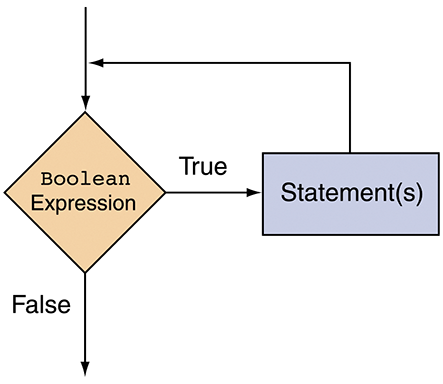
\includegraphics[scale=0.2]{Images/chapter04_whileLoop.png}
    \end{figure}
\end{frame}

\begin{frame}[fragile]{The while Loop}
    \begin{lstlisting}
// WhileLoop.java
public class WhileLoop {
    public static void main(String[] args) {
        int number = 1;
        while (number <= 5) {
            System.out.println("Hello");
            number++;
            }
        System.out.println("That's all");
        }
    }
    \end{lstlisting}
    Each repetition of a loop is known as an \violet{iteration}. This loop performs five iterations. I highly recommend you convince yourself this is true before moving on.
\end{frame}

\begin{frame}[fragile]{The while Loop}
    The while loop is known as a \violet{pretest loop} because it tests its boolean expression before each iteration. \\

    \vspace{1em}

    A while loop will never iterate if the boolean expression is false to start with. \\ 

    \vspace{1em}

    If a loop does not have a way of stopping, it is called an \violet{infinite loop}. Here is an example,
    \begin{lstlisting}
int number = 1;
while (number <= 5) {
    System.out.println("Hello");
    }
    \end{lstlisting}
\end{frame}

\begin{frame}[fragile]{The while Loop}
    Similar to the if statement, it's good practice to wrap loop statements around braces.
    \begin{lstlisting}[basicstyle=\ttfamily\footnotesize]
// Example of an infinite loop
int number = 1;
while (number <= 5) 
    System.out.println("Hello");
    number++;
    \end{lstlisting}
    To avoid the infinite loop we can write
    \begin{lstlisting}[basicstyle=\ttfamily\footnotesize]
// Example of a finite loop
int number = 1;
while (number <= 5) {
    System.out.println("Hello");
    number++;
    }
    \end{lstlisting}
\end{frame}

\begin{frame}[fragile]{The while Loop for Input Validation}
    The while loop can be used to create input routines that repeat until acceptable data is entered.

    When validating input, if an invalid value is entered a loop can require that the user reenter it as many times as necessary.
    \begin{lstlisting}
int number;
Scanner keyboard = new Scanner(System.in);
System.out.print("Type a number between 1 and 100: ");
number = keyboard.nextInt();
while (number < 1 || number > 100) {
    System.out.print("Invalid input. Reenter the number.");
    number = keyboard.nextInt();
    }
    \end{lstlisting}
\end{frame}

\subsection{do-while}
\begin{frame}[fragile]{The do-while Loop}
    The do-while loop is a \violet{posttest loop} because its boolean expression is tested after each iteration.

    In Java, the general idea is as follows.
    \begin{lstlisting}
do {
    Statement;
    Statement;
} while (BooleanExpression);
    \end{lstlisting}
\end{frame}

\begin{frame}[fragile]{The do-while Loop}
    Next are two snippets comparing the while and the do-while loop.
    \begin{lstlisting}
// while loop example
int x = 1;
while (x < 0) {
    System.out.println(x);
    }
    \end{lstlisting}

    \begin{lstlisting}
// do-while example
int x = 1;
do {
    System.out.println(x)
} while (x < 0);
    \end{lstlisting}

    Note that only the do-while loop will call the print statement.
\end{frame}

\subsection{for}
\begin{frame}{The for Loop}
    The \violet{for loop} is ideal for performing a known number of iterations. \\
    \vspace{1em}
    Loops can be classified as either conditional or \violet{count-controlled}. \\ 
    \vspace{1em}
    In conditional loops, we do not always know the number of iterations. \\ 
    \vspace{1em}
    In \violet{count-controlled} loops we know the \violet{exact number} of iterations.
\end{frame}

\begin{frame}{The for Loop}
A count-controlled loop must possess three elements:
\begin{enumerate}
    \item It must \violet{initialize} a control variable to a starting value.
    \item It must \violet{test} the control variable by comparing it to a maximum value. When the control variable reaches its maximum value, the loop terminates.
    \item It must \violet{update} the control variable during each iteration. This is usually done by incrementing the variable.
\end{enumerate}
The \textbf{for} loop is ideal for writing count-controlled loops.
\end{frame}

\begin{frame}[fragile]{The for Loop}
    The general form when using a \violet{for loop} is as follows.
    \begin{lstlisting}
for (Initialization; Test; Update) {
    Statement;
    Statement;
    // Place as many statements here as necessary.
    }
    \end{lstlisting}
And here is an example:
    \begin{lstlisting}
for (count = 1; count <= 5; count++) {
    System.out.println("Hello");
    System.out.println("The count is " + count + ".");
    }
    \end{lstlisting}
    In the previous example, the control variable is \violet{count}.
\end{frame}

\begin{frame}[fragile]{The for Loop}
\begin{lstlisting}
// Squares.java
public class Squares {
    public static void main(String[] args) {
        int number; // Loop control variable
        System.out.println("Number \t Number Squared");
        System.out.println("------------------------");
        for (number = 1; number <= 10; number++) {
            System.out.println(
                number
                + "\t\t"
                + number * number
                );
            }
        }
    }
\end{lstlisting}
\end{frame}

\begin{frame}[fragile]{The for Loop}
    Since the \textbf{for} loop tests its \textbf{boolean} expression before it performs an iteration, it is a \violet{pretest} loop. \\
    \vspace{1em}
    The next example is a \textbf{for} loop that will never iterate.
    \begin{lstlisting}
for (count = 11; count <= 10; count++) {
    System.out.println("Hello");
    }
    \end{lstlisting}
    Finally, you most likely want to avoid updating the control variable inside the loop.
    \begin{lstlisting}
for (x = 1; x <= 10; x++) {
    System.out.println(x);
    x++; // Avoid doing this
    }
    \end{lstlisting}
\end{frame}

\begin{frame}[fragile]{The for Loop}
We can also use other update statements which differ from the increment operator. For example,
    \begin{lstlisting}
for (number = 2; number <= 100; number += 2) {
    System.out.println(number);
    }
    \end{lstlisting}
    as well as
    \begin{lstlisting}
for (number = 10; number >= 0; number--) {
    System.out.println(number);
    }
    \end{lstlisting}
\end{frame}

\begin{frame}[fragile]{The for Loop}
    Not only may the control variable be initialized in the initialization expression, but also it may be declared there.
    \begin{lstlisting}
for (int number = 1; number <= 10; number++) {
    System.out.println(number + "\t\t" + number * number);
    }
    \end{lstlisting}
    When a variable is declared in the initialization expression of a for loop, the scope of the variable is limited to the loop.
    \begin{lstlisting}
for (int count = 1; count <= 10; count++) {
    System.out.println(count);
    }
System.out.println("count is now " + count); // ERROR!
    \end{lstlisting}
\end{frame}

\begin{frame}[fragile]{The for Loop}
    It is possible to execute more than one statement in the initialization expression and the update expression.
    \begin{lstlisting}
    int x, y;
    for (x = 1, y = 1; x <= 5; x++) {
        System.out.println(
            x
            + " plus " 
            + y 
            + " equals " 
            + (x + y)
            );
        }
    \end{lstlisting}
\end{frame}

\begin{frame}[fragile]{The for Loop}
    We can further modify the loop to execute two statements in the update expression.
    \begin{lstlisting}
int x, y;
for (x = 1, y = 1; x <= 5; x++, y++) {
    System.out.println(x + " plus " + y + " equals " + (x + y));
    }
    \end{lstlisting}
If you wish to combine multiple \textbf{boolean} expressions in the test expression, you must use the \red{\&\&} or \red{$\vert \vert$} operators.
\end{frame}

\section{Running Totals and Sentinel Values}
\subsection{Running Total}
\begin{frame}{Running Total}
    A running total is a sum of numbers that accumulates with each iteration of a loop. \\ 
    \vspace{1em}
    Programs that calculate the total of a series of numbers typically use two elements:
    \begin{enumerate}
        \item A loop that reads each number in the series.
        \item A variable that accumulates the total of the numbers as they are read.
    \end{enumerate}
\end{frame}

\begin{frame}[fragile]{Running Total}
    \begin{lstlisting}[basicstyle=\ttfamily\scriptsize]
import java.util.Scanner;
public class TotalSales {
   public static void main(String[] args) {
	   int days;
	   double sales;
	   double totalSales = 0.0;
	   Scanner keyboard = new Scanner(System.in);
	   System.out.print("Number of days: ");
	   days = keyboard.nextInt();
	   for (int count = 1; count <= days; count++) {
		   System.out.print("Enter day " + count + " sales: ");
		   sales = keyboard.nextDouble();
		   totalSales += sales;   // Add sales to totalSales. 
		   }
	   System.out.printf("Total sales are $%,.2f", totalSales);
	   }
    }
    \end{lstlisting}
\end{frame}

\subsection{Sentinel Values}
\begin{frame}[fragile]{Sentinel Values}
    Sometimes the user has a very long list of input values, and \violet{doesn’t know the exact number of items}. \\ 
    \vspace{1em}
    A technique that can be used in these situations is to \violet{ask the user} to enter a sentinel value at the end of the list. \\ 
    \vspace{1em}
    A \violet{sentinel value} is a special value that cannot be mistaken as a member of the list, and signals that there are no more values to be entered.
\end{frame}

\begin{frame}[fragile]{Sentinel Values}
\begin{lstlisting}[basicstyle=\ttfamily\scriptsize]
import java.util.Scanner;
public class TotalSales {
    public static void main(String[] args) {
        int points;
        int totalPoints = 0;
        String outString = "Enter game points or -1 to end: ";
        Scanner kb = new Scanner(System.in);
        System.out.print(outString);
        points = kb.nextInt();
        while (points != -1) {
            totalPoints += points;
            System.out.print(outString);
            points = kb.nextInt();
            }
        System.out.println("Total points are " + totalPoints);
        }
    }
    \end{lstlisting}
\end{frame}

\section{More on Loops, File Input and Output, and Random Numbers}
\subsection{Nested Loops}
\begin{frame}{Nested Loops}
    A loop that is inside another loop is called a nested loop. \\ 
    \vspace{1em}
    Nested loops are necessary when a task performs a repetitive operation and that task itself must be repeated.    
\end{frame}

\begin{frame}[fragile]{Nested Loops}
    \begin{lstlisting}[basicstyle=\ttfamily\footnotesize]
// Simulate the clock.
for (int hours = 1; hours <= 12; hours++) {
    for (int minutes = 0; minutes <= 59; minutes++) {
        for (int seconds = 0; seconds <= 59; seconds++) {
            System.out.printf(
                "%02d:%02d:%02d\n", 
                hours,
                minutes, 
                seconds
                ); 
            }
        }
    }
    \end{lstlisting}
In a console, the sequence of outputs would be 01:00:00, 01:00:01, 01:00:02, ..., 12:59:57, 12:59:58, 12:59:59.
\end{frame}

\begin{frame}{Nested Loops}
    Some comments on nested loops:
    \begin{enumerate}
        \item An inner loop goes through all of its iterations for each iteration of an outer loop.
        \item Inner loops complete their iterations before outer loops do.
        \item To get the total number of iterations of a nested loop, multiply the number of iterations of all the loops.
    \end{enumerate}
\end{frame}

\begin{frame}[fragile]{Nested Loops}
Here is another interesting example.
\begin{lstlisting}
final int NUM_STEPS = 10;
for (int r = 0; r < NUM_STEPS; r++) {
    for (int c = 0; c < r; c++) {
        System.out.print(" ");
        }
    System.out.println("#");
    }
\end{lstlisting}
\end{frame}

\subsection{Deciding Which Loop to Use}
\begin{frame}{Deciding Which Loop to Use}
\begin{enumerate}
    \item The while Loop \\
    This is a pretest loop, ideal when you do not want to loop if the \textbf{boolean} condition is false from the beginning or if you want to use a sentinel value to terminate the loop.
    \item The do-while Loop \\ 
    This is a posttest loop. Ideal when you want to iterate at least once.
    \item The for Loop \\ 
    This is a pretest loop that has built-in expressions for initializing, testing, and updating. It is ideal in situations where the exact number of iterations is known.
\end{enumerate}
\end{frame}

\subsection{File Input and Output}
\begin{frame}{File Input and Output}
    The Java API provides several classes that you can use for \violet{writing data} to a file and \red{reading data} from a file. \\
    \vspace{1em}
    To write data to a file, yo can use the \violet{PrintWriter} class and, optionally, the \violet{FileWriter} class. \\
    \vspace{1em} 
    To read data from a file, you can use the \red{Scanner} class and the \red{File} class.
\end{frame}

\begin{frame}{File Input and Output}
    The programs you have written so far require you to reenter data each time the program runs because data stored in variables and objects in RAM disappear once the program stops running. \\
    \vspace{1em}
    Data may be saved in a file, which is usually stored on a computer’s disk. \\
    \vspace{1em}
    The data can then be retrieved and used at a later time. \\
    \vspace{1em} 
    In general,
    \begin{enumerate}
        \item The file must be opened. When the file is opened, a connection is created between the file and the program.
        \item Data is then written to the file or read from the file. 
        \item When the program is finished using the file, the file must be closed.
    \end{enumerate}
\end{frame}

\begin{frame}{File Input and Output}
    The terms input file and output file are commonly used. \\
    \vspace{1em} 
    An input file is a file that a program reads data from. It is called an input file because the data stored in it serves as input to the program. \\ 
    \vspace{1em} 
    An output file is a file that a program writes data to. It is called an output file because the program stores output in the file. \\ 
    \vspace{1em}
\end{frame}

\begin{frame}{File Input and Output}
    In general, there are two types of files: text and binary. \\ 
    \vspace{1em}
    A text file contains data that has been encoded as text. These can be opened and viewed in a Text Editor (Notepad, Notepad++, etc). \\ 
    \vspace{1em}
    A binary file contains data that has not been converted to text and cannot be viewed with a text editor. \\ 
    \vspace{1em}
    In this course we only focus on text files by calling the Java input and output operations within the \textbf{java.io} package.
\end{frame}

\begin{frame}{The PrintWriter Class}
    To write data to a file you will create an instance of the \textbf{PrintWriter} class. \\
    \vspace{1em}
    The \textbf{PrintWriter} class allows you to open a file for writing. \\
    \vspace{1em}
    It also allows you to write data to the file using the same print and println methods that you have been using to display data on the screen. \\
    \vspace{1em}
    You pass the name of the file that you wish to open, as a string, to the \textbf{PrintWriter} class’s constructor.
\end{frame}

\begin{frame}[fragile]{The PrintWriter Class}
    For example, the following statement creates a \textbf{PrintWriter} object and passes the file name StudentData.txt to the constructor.    
    \begin{lstlisting}
import java.io.*;
public class PrintWriterExample {
	public static void main(String[] args) throws IOException {
		PrintWriter outputFile = new PrintWriter("Data.txt");
		outputFile.close();
		}
	}
    \end{lstlisting}
    These statements will create an empty file named StudentData.txt and establish a connection between it and the PrintWriter object that is referenced by outputFile.
\end{frame}

\begin{frame}[fragile]{The PrintWriter Class}
    You can pass a reference to a \textbf{String} object as an argument to the \textbf{PrintWriter} constructor.
    \begin{lstlisting}[basicstyle=\ttfamily\footnotesize]
import java.io.*;
import javax.swing.*;
public class ReferenceStringExample {
	public static void main(String[] args) throws IOException {
		String filename;
		filename = JOptionPane.showInputDialog("Enter the "
				+ "filename.");
		PrintWriter outputFile = new PrintWriter(filename);
		outputFile.close();
		}
	}
    \end{lstlisting}
\red{If the file that you are opening already exists, it will be erased and an empty file by the same name will be created.}
\end{frame}

\begin{frame}[fragile]{The PrintWriter Class}
    The \textbf{print} and \textbf{println} methods can be sued to write data to a file opened with the \textbf{PrintWriter} class.
    \begin{lstlisting}[basicstyle=\ttfamily\scriptsize]
// SongWriting.java
String filename = "SomeSong.txt";
PrintWriter outputFile = new PrintWriter(filename);
outputFile.println("And as you stay for the play, fantasy, has in store for you");
outputFile.println("A glowing light will see you through");
outputFile.println("It's your day, shining day, all your dreams come true");
outputFile.println("As you glide, in your stride with the wind, as you fly away");
outputFile.println("Give a smile, from your lips, and say");
outputFile.println("I am free, yes I'm free, now I'm on my way");
outputFile.close();
    \end{lstlisting}
\scriptsize{
Note you should always close files when finished with them. When a file is opened, the system creates one or more buffers (a small "holding section" of memory). The \textbf{close} method writes any unsaved data remaining in the file buffer.}
\end{frame}

\begin{frame}{Adding a throws Clause to the Method Header}
When an unexpected event occurs in a Java program, it is said that the program throws an exception. \\ 
\vspace{1em}
You can think of an exception as a signal indicating that the program cannot continue until the unexpected event has been dealt with. \\ 
\vspace{1em} 
For example, suppose you create a \textbf{PrintWriter} object and pass the name of a file to its constructor. \\
\vspace{1em} 
The \textbf{PrintWriter} object attempts to create the file, but unexpectedly, the disk is full and the file cannot be created. 
\end{frame}

\begin{frame}{Appending Data to a File}
    When you pass the name of a file to the \textbf{PrintWriter} constructor, and the file already exists, it will be erased and a new empty file with the same name will be created. \\ 
    \vspace{1em} 
    Sometimes you want to preserve an existing file and append new data to its current contents. \\ 
    \vspace{1em} 
    Appending to a file means writing new data to the end of the data that already exists in the file.
\end{frame}

\begin{frame}[fragile]{Appending Data to a File}
    To append data to an existing file, you first create an instance of the \textbf{PrintWriter} class. \\ 
    \vspace{1em} 
    You pass two arguments to the \textbf{PrintWriter} constructor: a string containing the name of the file, and the \textbf{boolean} value true.
    \begin{lstlisting}
FileWriter fwriter = new FileWriter("MyFriends.txt", true);
PrintWriter outputFile = new PrintWriter(fwriter);
outputFile.println("Bill");
outputFile.println("Steven");
outputFile.println("Sharon");
outputFile.close();
    \end{lstlisting}
\end{frame}

\begin{frame}[fragile]{Specifying File Location}
When you open a file you may specify its path along with its filename. \\ 
\vspace{1em} 
On a Windows computer, paths contain backslash characters. \\ 
\vspace{1em} 
For example, the path "E:\textbackslash \textbackslash Names.txt" specifies that Names.txt is in the root folder of drive E:. \\ 
\vspace{1em} 
The path "C:\textbackslash \textbackslash MyData \textbackslash \textbackslash Data.txt" specifies that Data.txt is in the \textbackslash \textbackslash MyData folder on drive C:. \\ 
\vspace{1em}
The next example shows how to create the file "PriceList.txt" in the root folder of drive C.
\begin{lstlisting}
PrintWriter outputFile = new PrintWriter("C:\\PriceList.txt");
\end{lstlisting}
\end{frame}

\begin{frame}[fragile]{Reading Data from a File}
    Recall that the \textbf{Scanner} class allows us to read input from the keyboard. \\ 
    \vspace{1em} 
    The \textbf{Scanner} class can also read an input from a file.
    \begin{lstlisting}
File myFile = new File("Customers.txt");
Scanner inputFile = new Scanner(myFile);
// Can now call Scanner methods on inputFile here
inputFile.close();
    \end{lstlisting}
This means you can then call \textbf{Scanner} methods, such as \textbf{nextLine}.
\end{frame}

\subsection{Generating Random Numbers with the Random Class}
\begin{frame}{Random Numbers}
     Java provides the \textbf{Random} class that you can use to generate random numbers. Random numbers can be used in a variety of ways.
     \begin{enumerate}
         \item Computer games that let the player roll dice use random numbers to represent the values of the dice.
         \item Selecting data randomly for statistical analysis.
         \item Computer security to encrypt sensitive data.
     \end{enumerate}
\end{frame}

\begin{frame}[fragile]{Random Numbers}
   \begin{lstlisting}[basicstyle=\ttfamily\scriptsize]
// import java.util.Scanner and java.util.Random;
int number1, number2, sum, userAnswer;
Scanner kb = new Scanner(System.in);
// Random randomNumbers: declare variable of type Random
// new Random(): create an instance of the Random class
// assign the address of the Random class to the variable randomNumbers
Random randomNumbers = new Random();
number1 = randomNumbers.nextInt(100);
number2 = randomNumbers.nextInt(100);
System.out.print(number1 + " + " + number2 + " = ? ");
sum = number1 + number2;
userAnswer = kb.nextInt();
if (userAnswer == sum) {
    System.out.println("Correct!");
    }
else {
    System.out.println("The correct answer is " + sum);
    }
kb.close();
   \end{lstlisting} 
\end{frame}

\end{document}

